\documentclass{beamer}
 
\usepackage[utf8]{inputenc}
\usepackage[serbian]{babel}
 
\usetheme{Copenhagen}
 
\title{Predviđanje funkcije proteina metodama binarne klasifikacije}
\author{Anja Bukurov}
\institute{Matematički fakultet}
\date{26.06.2019}
 
 
 
\begin{document}
 
\frame{\titlepage}

 
\begin{frame}
	\frametitle{Sadržaj}
	\tableofcontents
\end{frame}


\section{Motivacija}
\begin{frame}{Motivacija}
	\frametitle{Motivacija}

	\begin{itemize}
		\item Svake godine sekvencira se veliki broj novih genoma
		
		\item Eksperimentalno određivanje funkcije je skup i spor proces
		
		\item Ulaže se veliki trud u razvoj računarskih metoda koji mogu da predvide funkciju proteina
		
		\item Mnogi postojeći pristupi koriste informacije o sekvenci proteina na neki način
		
		
	\end{itemize}

\end{frame}
 

\section{Uvodni pojmovi}

\subsection{Proteini}
\begin{frame}{Sinteza proteina}
	\frametitle{Sinteza proteina}

	\begin{itemize}
		\item Makromolekuli koji igraju mnoge kritične uloge u organizmu
		
		\item Sačinjavaju više od 50\% suvog dela ćelije i važni su za njenu izgradnju i funkcionisanje
		
		\item Sinteza proteina sastoji se iz dva koraka: transkripcije i translacije
		
	\end{itemize}

	\begin{figure}
		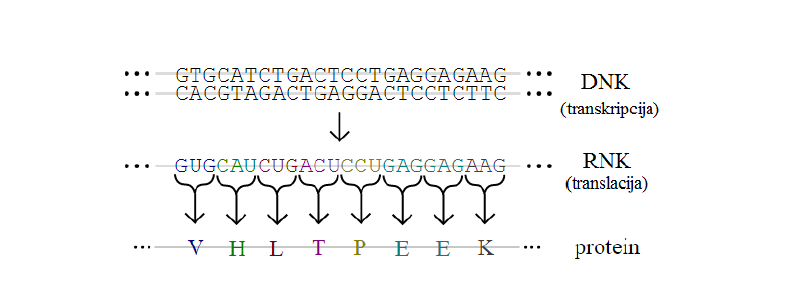
\includegraphics[width=\textwidth]{../Tekst/Figures/protein_synthesis.png}
	\end{figure}

\end{frame}

\begin{frame}{Struktura proteina}
\frametitle{Struktura proteina}

	\begin{itemize}
		\item Proteini su izgrađeni od 20 standarnih aminokiselina
		
		\item Aminokiseline su jedinjenja koja sadrže jednu karboksilnu grupu, jednu amino grupu i bočni R-lanac
		
		\item Dve aminokiseline se vezuju peptidnom vezom koja se formira između ugljenika iz karboksilne i azota iz amino grupe
		
		\item Redosled aminokiselina jedinstven je za svaki protein i čini njegovu primarnu strukturu
	
	\end{itemize}
	
\end{frame}
 

\subsection{Binarna klasifikacija}
\begin{frame}{Binarna klasifikacija}
	\frametitle{Binarna klasifikacija}
	
	\begin{itemize}
		\item Zadatak dodeljivanja objekta jednoj od dve predefinisane kategorije
		
		\item Svaki klasifikator koristi algoritam za učenje kako bi odredio model koji najbolje odgovara vezi između skupa atributa i kategorija ulaznih podataka
		
		\item Model bi trebalo da odgovara ulaznim podacima i da tačno predviđa klasu slogova koje ranije nije video
	\end{itemize}
	
\end{frame}

\begin{frame}{Metod potpornih vektora}
	\frametitle{Metod potpornih vektora}
	
	\begin{itemize}
		\item Tehnika zasnovana na pronalasku razdvajajuće hiperravni
		\item Sve instance iste klase treba da se nađu sa iste strane hiperravni
		
		\item Takvih ravni množe biti mnogo, ali nisu sve podjednako dobre
		\item Traži se ona koja maksimizuje rastojanje između instanci dve klase
	\end{itemize}
\end{frame}


\begin{frame}{Metod potpornih vektora}
	\frametitle{Metod potpornih vektora}
	
	\begin{itemize}
		\item Tehnika zasnovana na pronalasku razdvajajuće hiperravni
		\item Sve instance iste klase treba da se nađu sa iste strane hiperravni
		
		\item Takvih ravni množe biti mnogo, ali nisu sve podjednako dobre
		\item Traži se ona koja maksimizuje rastojanje između instanci dve klase
	\end{itemize}
\end{frame}


\begin{frame}{Logistička regresija}
	\frametitle{Logistička regresija}
	
	\begin{itemize}
		\item Statistički zasnovana metoda
		\item Zadatak je pronaći hiperravan koja deli podatke tako da sa jedne strane budu instance iste klase
		\item Računa se verovatnoća da instanca pripada jednoj od klasa 
		\item Verovatnoća je veća što je instanca dalja od hiperravni sa odgovarajuće strane
	\end{itemize}
\end{frame}

 
 
\begin{frame}{Slučajne šume}
	\frametitle{Slučajne šume}
	
	\begin{itemize}
		\item Metod asambla dizajniran za stabla odlučivanja
		\item Čvorovi stabla sadrže pitanja, a grane su odgovori na njih
		\item Listovi sadrže oznake klasa
		\item Klasifikacija se vrši glasanjem - svako od stabla klasifikuje instancu, a prebrojavanjem se odlučuje koja je klasa
	\end{itemize}
\end{frame}


\section{Implementacija}
\subsection{Predstavljanje proteina i funkcija}
\begin{frame}{Predstavljanje proteina i funkcija}
	\frametitle{Predstavljanje proteina}
	\begin{itemize}
		\item Aminokiseline su u računaru predstavljene kao jedan karakter 
		\item Sekvenca je predstavljena kao niska aminokiselina
		\item Protein je predstavljen kao niz dimenzije $20^3$ gde svaki element predstavlja broj pojavljivanja odgovarajućeg trigrama
		\item Trigram se preslikava u broj po formuli 
		
		$$trigram\_broj = ak_1 * 20^2 + ak_2 * 20 + ak_3$$
		
		pri čemu svaka aminokiselina ima dodeljen broj $ak_i$ iz intervala $[0, 19]$
	\end{itemize}
\end{frame}

\begin{frame}{Predstavljanje proteina i funkcija}
	\frametitle{Predstavljanje funkcija}
	\begin{itemize}
		\item Sistem za predstavljanje funkcije proteina koji se
		trenutno najviše koristi je \textit{Gene Ontology}
		
		\item Funkcije proteina podeljene su na tri
		ontologije: biološki procesi (BPO), molekulske funkcije (MFO) i ćelijske komponente (CCO).
		
		\item Ontologija je predstavljena kao usmereni acikli£ki graf gde su čvorovima pridruženi nazivi funkcija, a grane koje ih povezuju definišu relaciju \textit{is\_a}
		
		\item Svaki čvor ima specifičniju funkciju od roditeljskog čvora
	
		\item U korenu svake ontologije nalazi se funkcija sa nazivom te ontologije, a u listovima su najspecifičnije fukcije
	\end{itemize}
\end{frame}



\begin{frame}{Skupovi za obučavanje i evaluaciju}
	\frametitle{Skupovi za obučavanje i evaluaciju}
	\begin{itemize}
		\item Početni skup 20960 proteina podeljen je na trening i test skup
		
		\item Za trening je izdvojeno 20860 proteina koji su korišćeni za obučavanje pojedinačnih binarnih modela
		
		\item Svaki binarni model predstavlja najbolji od nekoliko modela koji se razlikuju po korišćenim parametrima, a odabrani su na osnovu rezultata postignutih na podskupu trening skupa koji je izdvojen za validaciju
		
		\item Na test skupu od 100 proteina upoređeni su konačni prediktori čiji odgovor predstavlja uniju odgovora svih binarnih klasifikatora 
	\end{itemize}
\end{frame}

\section{Rezultati}
\begin{frame}{Rezultati}
	\frametitle{Rezultati}
	
\end{frame}


\section{}
\begin{frame}
	\centering \Large Hvala na pažnji!
\end{frame}

\end{document}

